\section{Profile-based algorithm}\label{sec:old_method}

The Profile-based algorithm classifies clouds by individual profiles \citep{pirloagaGroundBasedMeasurementsCloud2022, nomokonovaStatisticsCloudsTheir2019, kneifelMultiyearCloudPrecipitation2022}. The PBA uses the target classification (TC) from Cloudnet to classify sequences of pixels with height. For each time step, vertical sequences of pixels in TC are classified as follow: 

\begin{enumerate}
	
	\item Cloud layer criteria: More than 3 consecutive hydrometeor pixels (38-153 m) \citep{nomokonovaStatisticsCloudsTheir2019} are considered a cloud layer.
	
	\begin{enumerate}
		\item Liquid criteria: Sequence of only "Droplets" and "Drizzle \& Droplets" pixels
		
		\item Ice criteria: Sequence of only "Ice" pixels
		
		\item Mixed-Phase criteria: Sequence of only "Droplets", "Ice", "Ice \& Droplets", "Melting ice", "Melting \& droplets", "Drizzle and droplets" pixels
		
		\item Rain criteria: For Liquid or Mixed-Phase clouds, if more than 1 pixel of "Drizzle or rain" is found below the cloud layer, then it is considered as a precipitating layer. Thus, this cloud layer is then classified as Precipitating Liquid cloud or Precipitating Mixed-Phase cloud.
		
	\end{enumerate}
	
	\item Multilayer classification
	
	\begin{enumerate}
		
		\item Multi-layer criteria: More than 4 pixels (64-255 m) \citep{pirloagaGroundBasedMeasurementsCloud2022} of any combination of "Clear sky", "Aerosol", "Insect" and "Aerosol \& insect" between cloud layers. Otherwise, it's a single layer cloud. 
		
	\end{enumerate}
	
\end{enumerate}

\section{Pixel dilatation}\label{sec:dilation}

The dilation method consists in expanding the ones in the cloud mask to connect the closest groups of hydrometeors, which are likely to belong to the same cloud. The dilatation follows the scheme below, where hydrometeor pixels are represented in blue. Left image represents the original hydrometeor pixels where two groups of clouds were identified. Thus, a dilatation of 1 pixel is applied in all directions, represented by the red pixels in the right image. Therefore, the dilation process will unite these groups with at least 2 pixels of separation distance. Since they are connected, the cloud classification algorithm will save the coordinates of these cloud pixels in just one group (not two, as previously identified).

\begin{figure}[H]
	\centering
	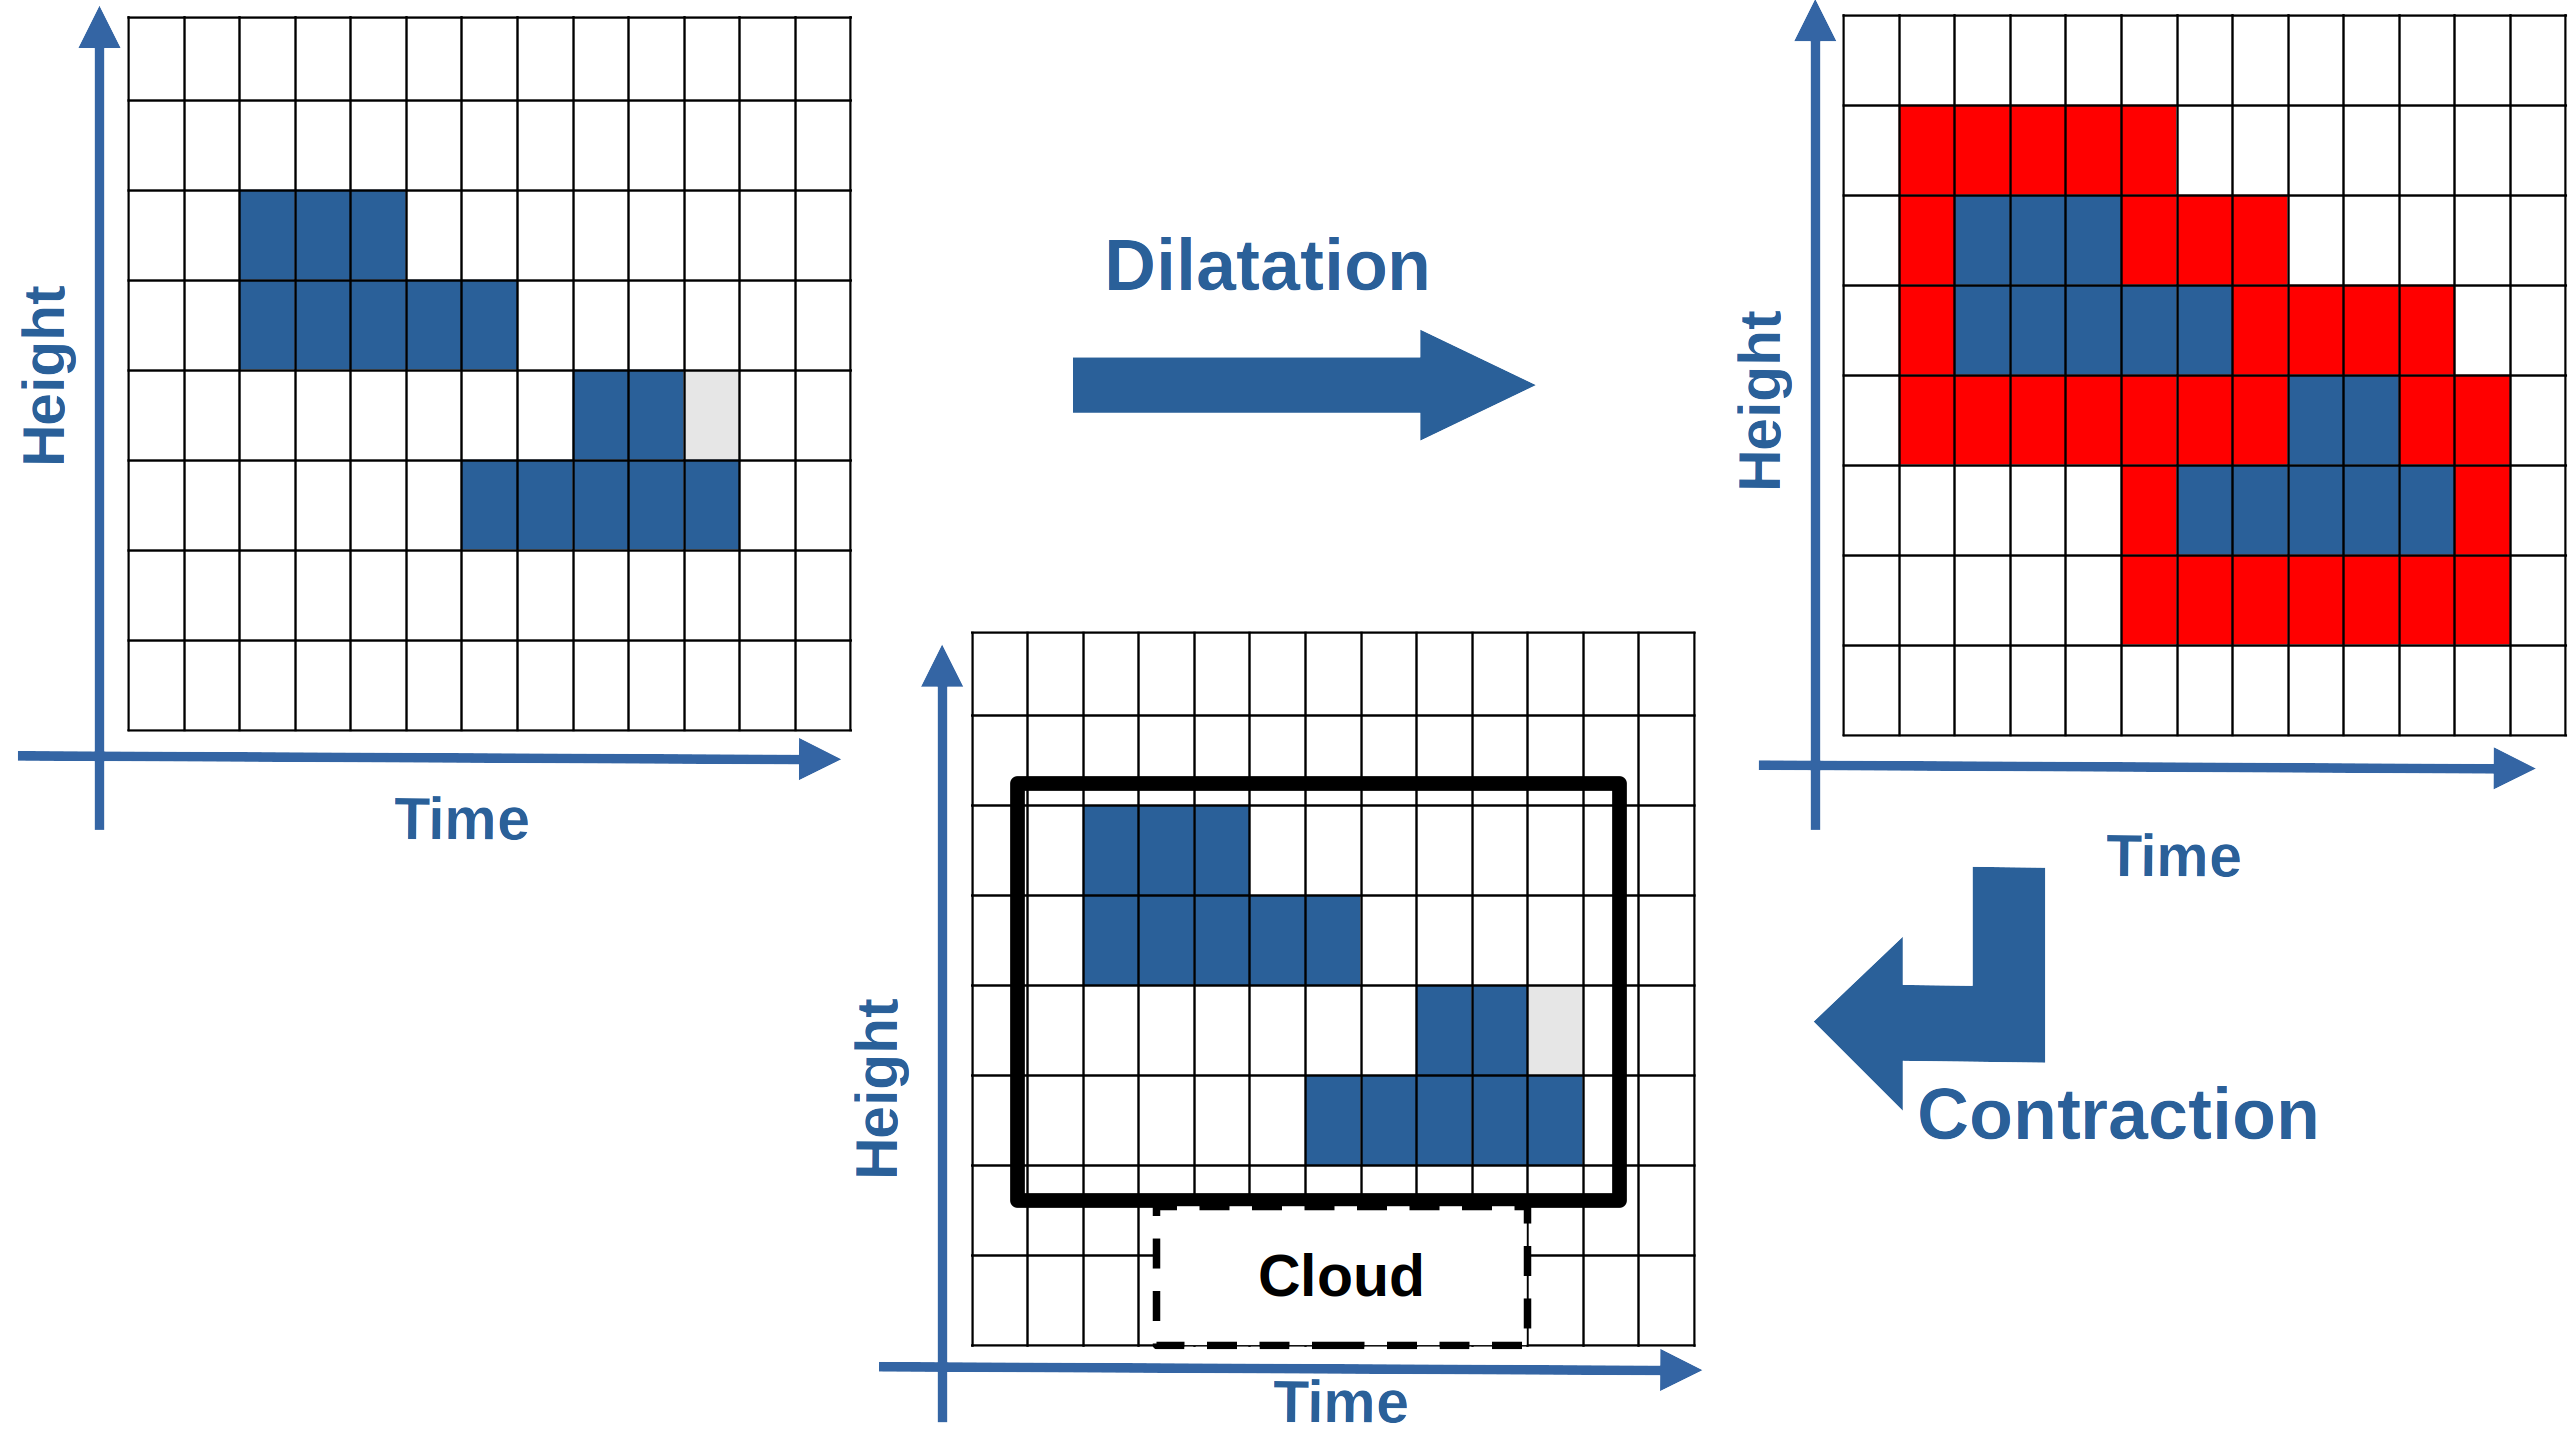
\includegraphics[width=.7\textwidth]{./figures/scheme_dilatation}
	\caption{Pixel dilatation and pixel contraction illustration. Left panel shows two hydrometeor groups. Right panel still shows these two clouds and the dilated pixels in red. Since these clouds are connected, the classification algorithm will understand there is only one cloud. Bottom panel shows the result of the pixel contraction, returning cloud pixels to its original position}
	\label{fig:dilatation}
\end{figure}

Next, a contraction process is done to return the coordinates of true hydrometeors to the original position. The contraction will remove the fake coordinates of hydrometeor (pixels in red on the above figure). In order to illustrate the method, the left panel of Figure \ref{fig:cluster_identification} shows the Cloudnet hydrometeor classification product (on 11 February 2021), while the right panel shows all hydrometeors clusters. Groups inside the black dashed lines are considered clusters and will be classified into cloud types. Additionally, clusters that are very close to each other will be merged.

\begin{figure}[H]
	\centering
	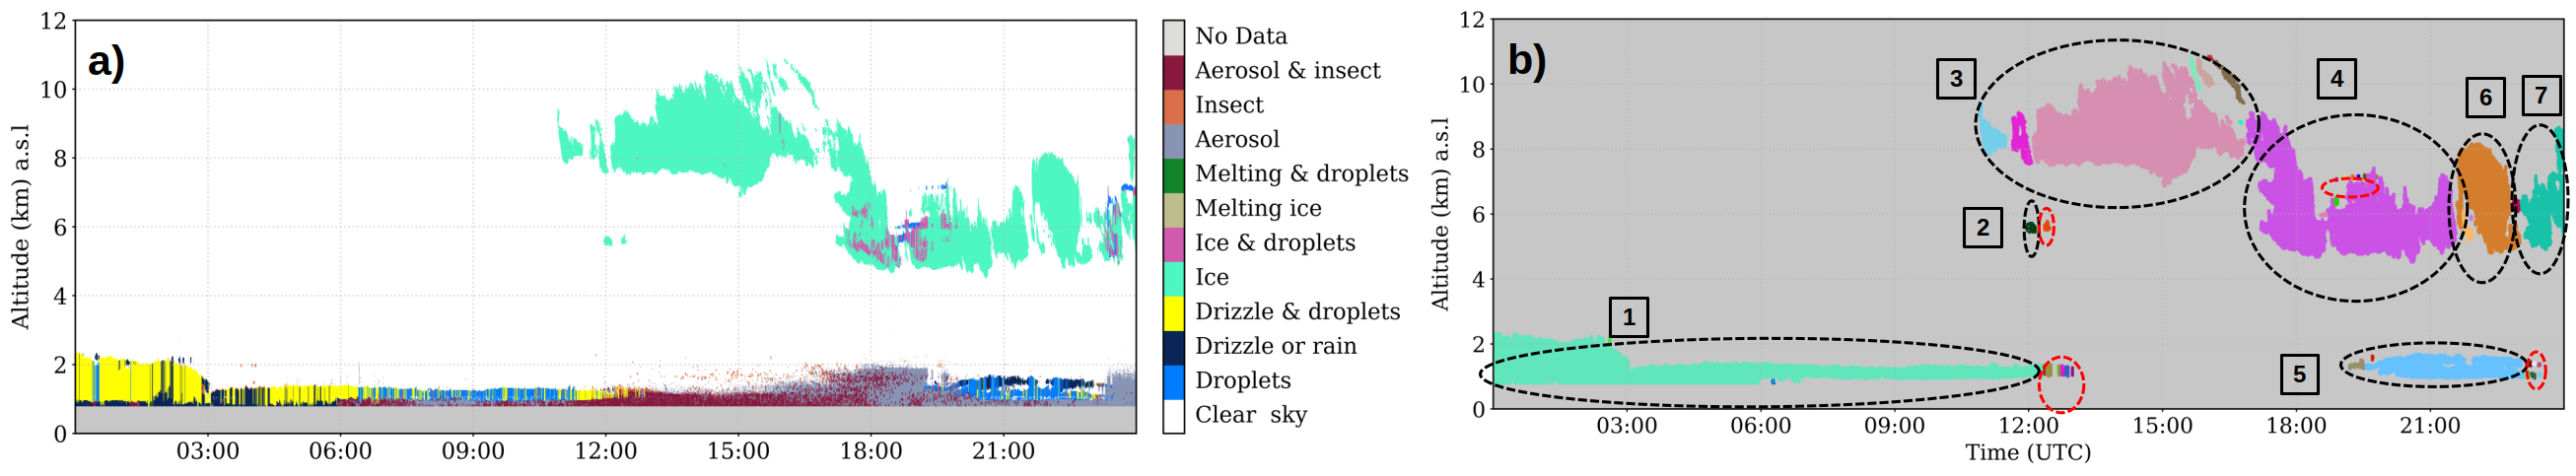
\includegraphics[width=.95\textwidth]{./figures/20210211_cloud_identification}
	\caption{Cloud cluster identification by Cloudnet target classification on 11 February 2021. (a) Target classification, which shows particles typing in time and altitude. (b) Cloud clusters identified in black (dashed lines) and noise (less than 100 pixels connected) by red, dashed lines}
	\label{fig:cluster_identification}
\end{figure}
